Consider the data on national parks in Exercise 1.27.
\begin{enumerate}[label= (\alph*)]
    \item Comment on any possible outliers in a scatter plot of the original variables.
    
    The scatter plot of the data is below. We only have 15 observations, so the sample size is small. In the x-drection, park size in acres, it looks like there's one observation, corresponding to Yellowstone, which has a very large size of 2219.8 acres. In the y-direction, number of visitors in millions, there also appears to be a park with a very large numer of visitors, corresponding to Great Smoky (9.19 million).

    \begin{center}
        \begin{figure}[H]
            \centering
            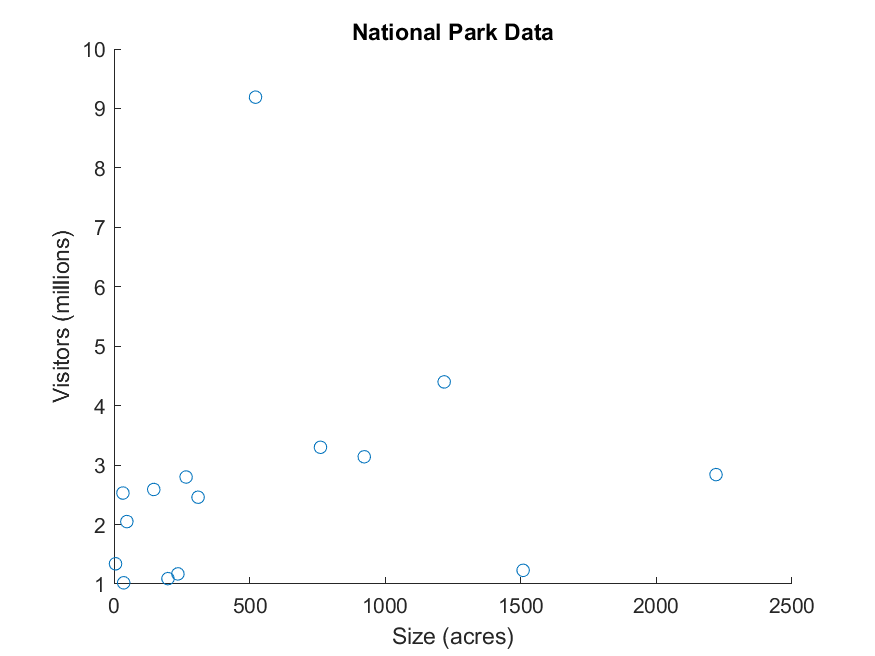
\includegraphics[scale=0.6]{./matlab/chapter-4/sol4.40.a.png}
        \end{figure}
    \end{center}

    \item Determine the power transformation $\hat{\lambda}_{1}$ the makes the $x_{1}$ values approximately
    normal. Construct a Q-Q plot of the transformed observations.

    For park size in acres, $x_{1}$, the optimal Box-Cox power transformation value found was $\hat{\lambda}_{1} = 0.1904$.
    I rounded that to 0.2, so $x_{1}^{\prime} = x_{1}^{\hat{\lambda}_{1}} = x_{1}^{0.20}$. This transformation increased the Q-Q correlation coefficient to 0.9909, which is larger than the critical point values of 0.9110, 0.9392, and 0.9506 who represent the 0.01, 0.05, and 0.10 levels, respectively, for a sample size of 15.
    Because of this the data would be considered normally distributed at all the usual levels.
    Below are the results of the power transformation and the Q-Q plots of the transformed data.
    For only having 15 observations, the Q-Q plot of the transformed data looks fairly linear.

    \begin{center}
        \begin{figure}[H]
            \centering
            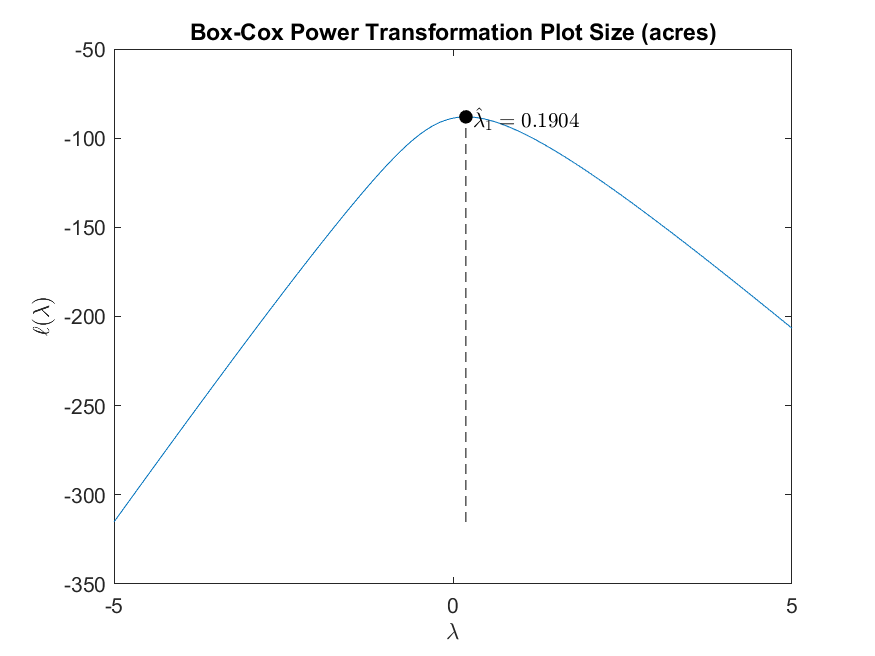
\includegraphics[scale=0.4]{./matlab/chapter-4/sol4.40.power.1.png}
        \end{figure}
    \end{center}
    
    \begin{center}
        \begin{figure}[H]
            \centering
            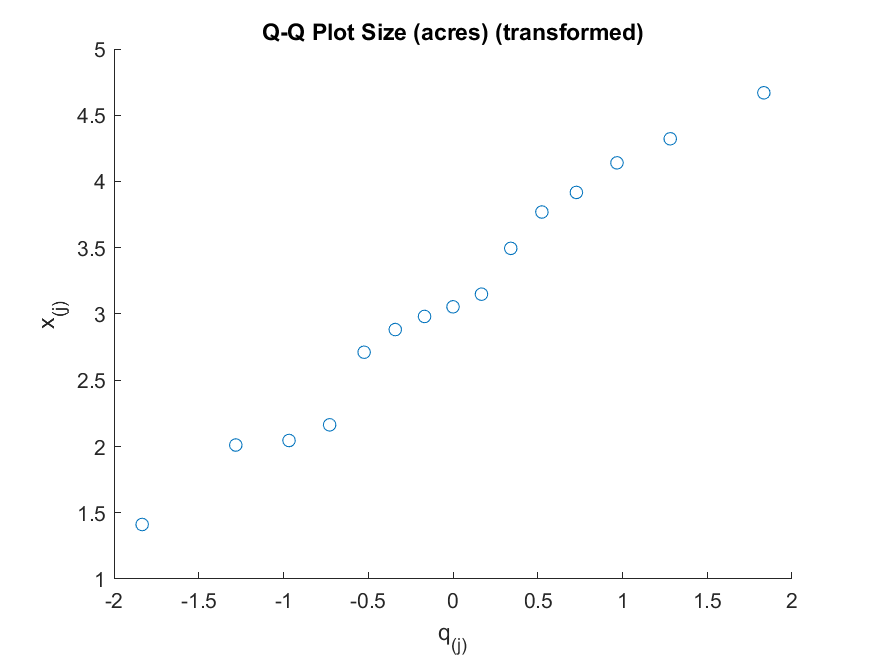
\includegraphics[scale=0.4]{./matlab/chapter-4/sol4.40.qq.tr.1.png}
        \end{figure}
    \end{center}


    \item Determine the power transformation $\hat{\lambda}_{2}$ the makes the $x_{2}$ values approximately
    normal. Construct a Q-Q plot of the transformed observations.


    For number of visitors in millions, $x_{2}$, the optimal Box-Cox power transformation value found was $\hat{\lambda}_{2} = -0.3507$.
    I rounded that to -0.35, so $x_{1}^{\prime} = x_{2}^{\hat{\lambda}_{2}} = x_{2}^{-0.35}$. This transformation increased the Q-Q correlation coefficient to 0.9675, which is larger than the critical point values of 0.9110, 0.9392, and 0.9506 who represent the 0.01, 0.05, and 0.10 levels, respectively, for a sample size of 15.
    Because of this the data would be considered normally distributed at all the usual levels.
    Below are the results of the power transformation and the Q-Q plots of the transformed data.
    The transformed Q-Q plot doesn't look strongly linear, but our sample size is only 15, so the bar isn't very high.

    \begin{center}
        \begin{figure}[H]
            \centering
            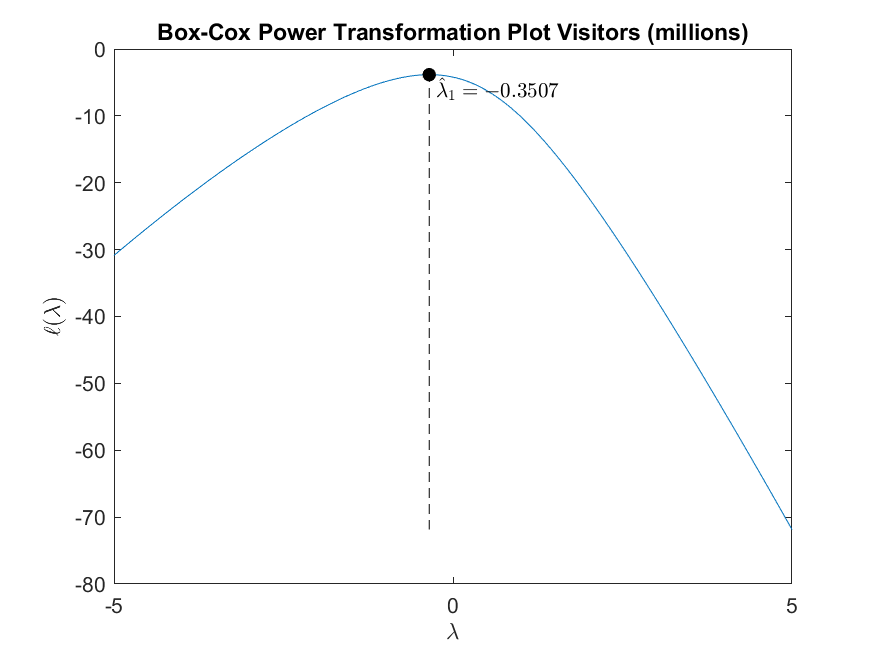
\includegraphics[scale=0.4]{./matlab/chapter-4/sol4.40.power.2.png}
        \end{figure}
    \end{center}
    
    \begin{center}
        \begin{figure}[H]
            \centering
            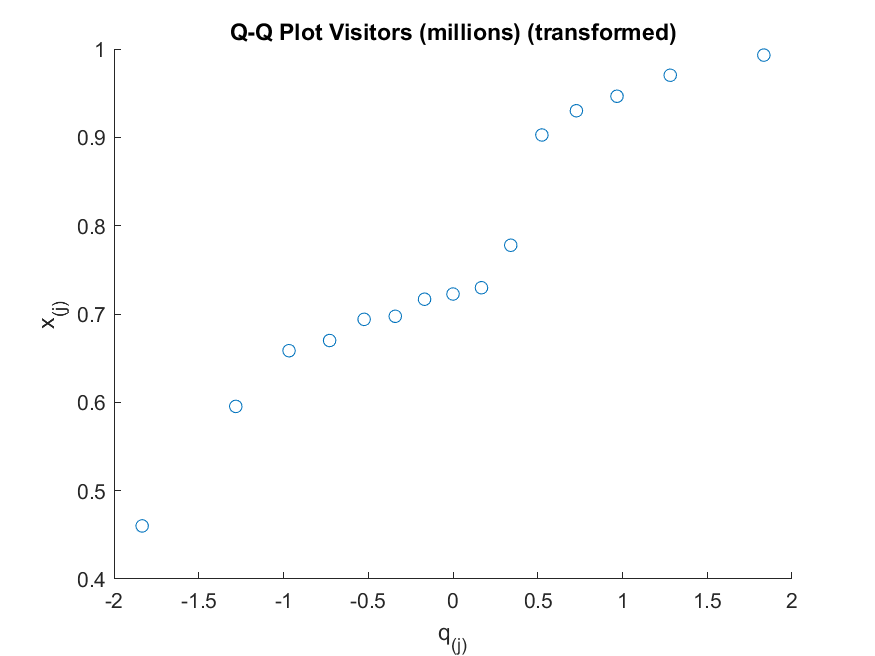
\includegraphics[scale=0.4]{./matlab/chapter-4/sol4.40.qq.tr.2.png}
        \end{figure}
    \end{center}

    \item Determine the power transformation for approximate bivariate normality using (4--40).
    
    The optimum found was at $\left(\hat{\lambda}_{1}, \hat{\lambda}_{2}\right) = (0.1678, -0.3423)$. These values are close to those found in part (b) and (c), where the result of optimizing the univariate transform using Box-Cox was $\left(\hat{\lambda}_{1}, \hat{\lambda}_{2}\right) = (0.1904, -0.3507)$. The contour and surface plot for $\ell \left(\lambda_{1}, \lambda_{2}\right)$ is below.

    \begin{center}
        \begin{figure}[H]
            \centering
            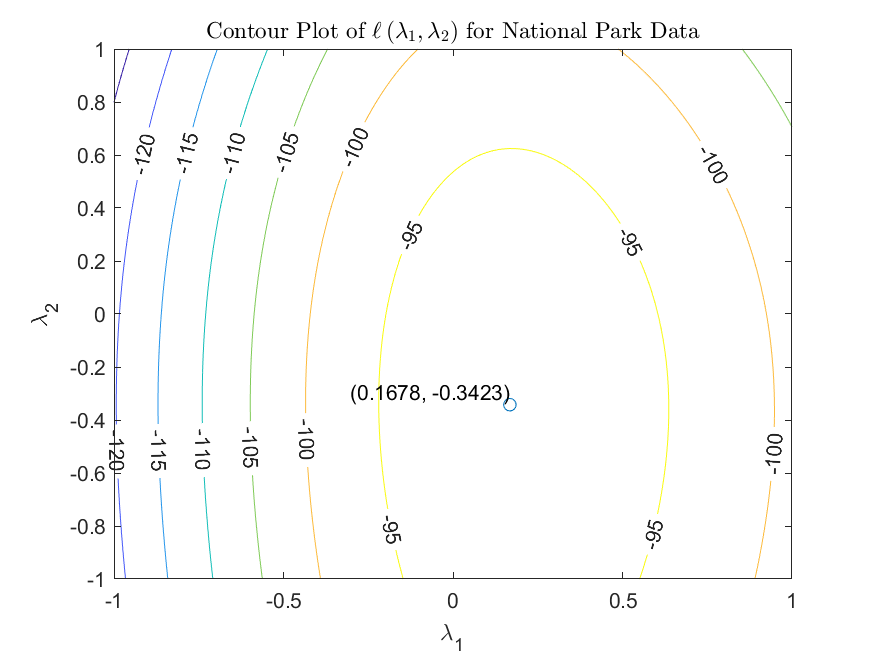
\includegraphics[scale=0.6]{./matlab/chapter-4/sol4.40.d.contour.png}
        \end{figure}
    \end{center}
    
    \begin{center}
        \begin{figure}[H]
            \centering
            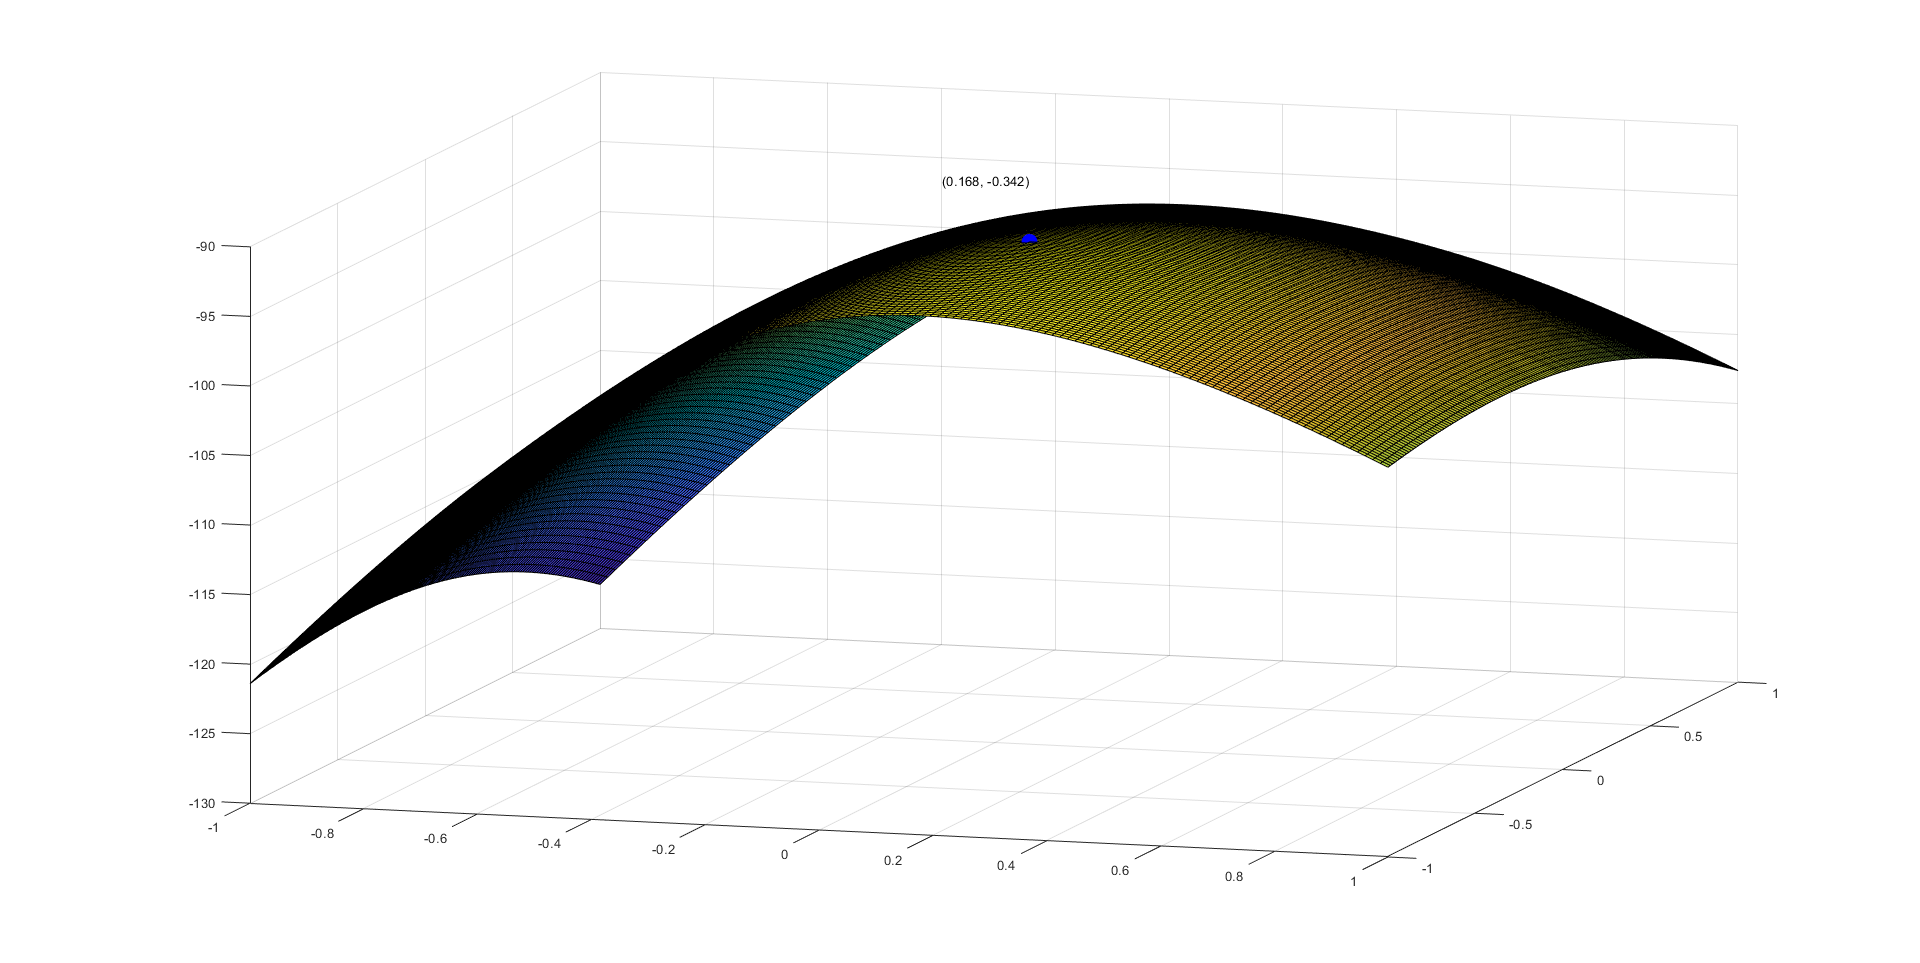
\includegraphics[scale=0.3]{./matlab/chapter-4/sol4.40.d.surf.png}
        \end{figure}
    \end{center}
    
\end{enumerate}